\documentclass{beamer}

\mode<presentation> {
\usetheme{Madrid}
}

\usepackage{graphicx}
\usepackage{booktabs}
\usepackage{polski}
\usepackage[polish]{babel}
\usepackage[utf8]{inputenc}
\usepackage[T1]{fontenc}
\usepackage[utf8]{luainputenc}
\usepackage{pgfgantt}
\usepackage{caption}
\usepackage{mwe}

% Strona tytułowa
\usepackage{pgfplots}
\usepackage{siunitx}
\usepackage{paracol}
\usepackage{gensymb}

% Pływające obrazki
\usepackage{float}
\usepackage{svg}
\usepackage{graphicx}
\usepackage{subfig}


\sisetup{group-digits=true,
        %  group-four-digits=true,
        round-precision=4,
        group-separator={},
        output-decimal-marker={,}}

\DeclareCaptionFormat{citation}{%
   \ifx\captioncitation\relax\relax\else
     \captioncitation\par
   \fi
   #1#2#3\par}
\newcommand*\setcaptioncitation[1]{\def\captioncitation{\tiny{\textit{Źródło:}~#1}\medskip}\normalsize}
\let\captioncitation\relax
\captionsetup{format=citation,justification=centering}

\usetikzlibrary{pgfplots.groupplots}
\sisetup{detect-weight,exponent-product=\cdot,output-decimal-marker={,},per-mode=symbol,binary-units=true,range-phrase={-},range-units=single}

%wymiar tekstu
\def\figurename{Rys.}
\def\tablename{Tab.}

%----------------------------------------------------------------------------------------
%	TITLE PAGE
%----------------------------------------------------------------------------------------

\title[SAG - Projekt]{Systemy Agentowe}

\author[Konieczka, Poturała, Sikora]{Maria Konieczka \and Alicja Poturała \and Jakub Sikora} 

\date{15 czerwca 2020}
\institute[]{Planowanie pracy w fabryce\\Prowadzący: dr inż. Dominik Ryżko}

\AtBeginSection[]
{
    \begin{frame}[plain, noframenumbering]
        \frametitle{Agenda}
        \tableofcontents[currentsection]
    \end{frame}
}

\begin{document}

\begin{frame}
    \titlepage
\end{frame}

\begin{frame}
    \frametitle{Agenda}
    \tableofcontents
\end{frame}

\section{Wprowadzenie w problem}
\begin{frame}
    \frametitle{Problem planowania sekwencji}
    \textbf{Cel}: znaleźć taką sekwencję produktów, która minimalizuje koszt fabryki.\\
    \medskip    
    Założenia:
    \begin{itemize}
        \item fabryka podzielona jest na \emph{n} komórek,
        \item każdy produkt musi przejść przez każdą komórkę,
        \item każda komórka może nadać produktowi jedną z \emph{m} cech,
        \item z każdą komórką związana jest funkcja kosztu,
        \begin{itemize}
            \item związany z~samym nadaniem cechy,
            \item związany z~poprzednią nadaną cechą, każda zmiana cechy zwiększa koszt,
        \end{itemize} 
        \item minimalizujemy koszt globalny, czyli sumę wszystkich kosztów lokalnych.
    \end{itemize}
\end{frame}

\section{Algorytm agentowy}
\begin{frame}
    \frametitle{Domena problemu}
    \begin{center}
        $ \big \langle P, O, S, A_{g}, f \big \rangle$
    \end{center}
    gdzie 
    \begin{itemize}
        \item $P$ to zbiór możliwych produktów,
        \item $O$ to zbiór zamówień złożony z~produktów z~$P$,
        \item $S$ to sekwencja produktów $P$,
        \item $A_{g} = \{1, \dots, l\}$ to zbiór agentów (komórek produkcji),
        \item $f = \{c_{i}\}$ jest zbiorem funkcji kosztu, reprezentującym fabrykę, każdemu agentowi $i \in A_{g}$ odpowiada funkcja kosztu $c_{i}$
    \end{itemize}
\end{frame}
\begin{frame}
    \frametitle{Pareto-optymalność rozwiązania}
    \begin{block}{\textbf{Pareto-optymalność a optymalność globalna}} Sekwencja globalnie optymalna, będzie pareto-optymalna dla jednego z~agentów w systemie. Możemy wykorzystać ten fakt do określenia zbioru negocjacyjnego $NS$ czyli zbioru sensownego do proponowania.
    \end{block}

    \begin{block}{
    \textbf{Agent $i$ może proponować tylko sekwencję pareto-optymalną}} Dzięki zauważeniu tej zależności, możemy ograniczyć przeszukiwaną dziedzinę do rozwiązań pareto-optymalnych dla któregoś z~agentów. Każdy z~agentów może samodzielnie określić swój zbiór $NS$ w~sposób niezależny od innych, co umożliwia zrównoleglenie obliczeń.
    \end{block}

\end{frame}

\begin{frame}
    \frametitle{Planowanie jako negocajcje w systemie agentowym}
    \begin{figure}
        \centering
        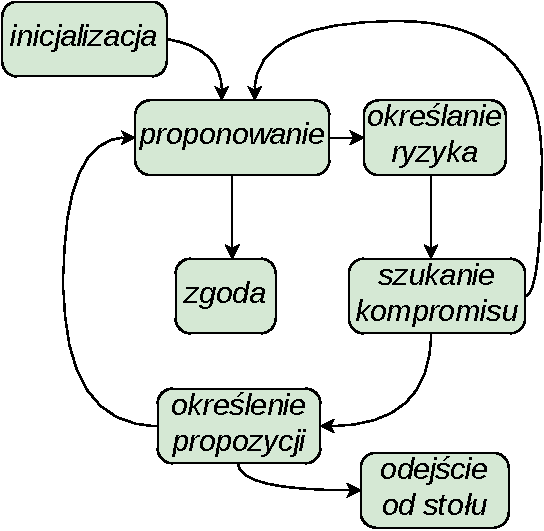
\includegraphics[width=0.6\columnwidth]{figures/SAG-Negotiation-Prezentacja.pdf}
        \label{fig:negocjacje}
    \end{figure}
\end{frame}

\section{Implementacja}
\begin{frame}
    \frametitle{Smart Python Agent Development Environment}
    Cechy biblioteki SPADE:
    \begin{itemize}
        \item oparta o~język Python 3.6,
        \item asynchroniczna komunikacja,
        \item wspiera standard FIPA,
        \item korzysta z~protokołu XMPP,
        \item model agenta oparty o~zachowania.
    \end{itemize}
\end{frame}

\begin{frame}
    \frametitle{Dekompozycja na agenty}
    \begin{figure}
        \centering
        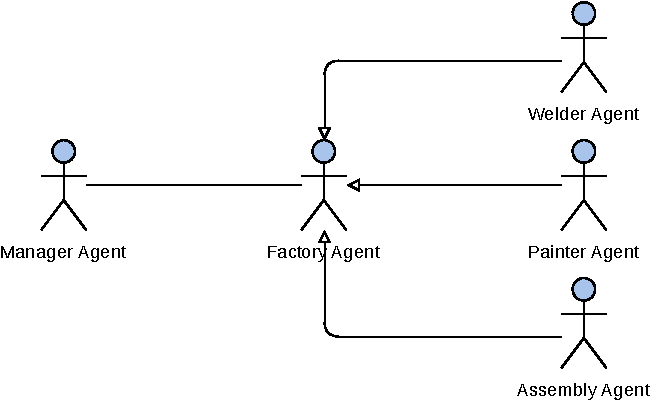
\includegraphics[width=0.95\columnwidth]{figures/SAG-Agents.pdf}
        \label{fig:agenci}
    \end{figure}
\end{frame}

\begin{frame}
    \frametitle{Dekompozycja na zachowania}
    \begin{figure}[!ht]
        \subfloat{%
            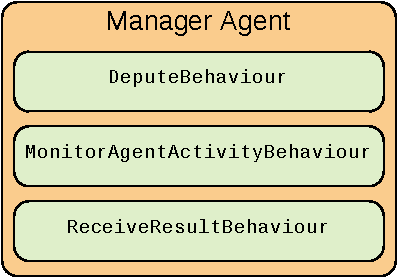
\includegraphics[width=0.55\columnwidth]{figures/SAG-Manager-Behaviours.pdf}
        }
        \subfloat{%
            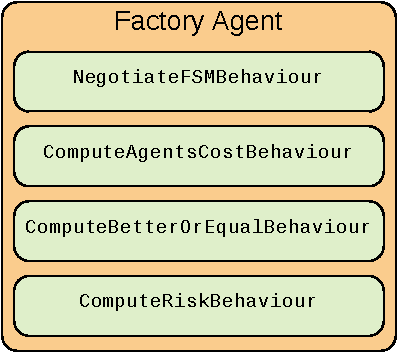
\includegraphics[width=0.45\columnwidth]{figures/SAG-Factory-Behaviours.pdf}
        }
    \end{figure}
\end{frame}

\begin{frame}
    \frametitle{Implementacja algorytmu negocjacji}
    \begin{figure}
        \centering
        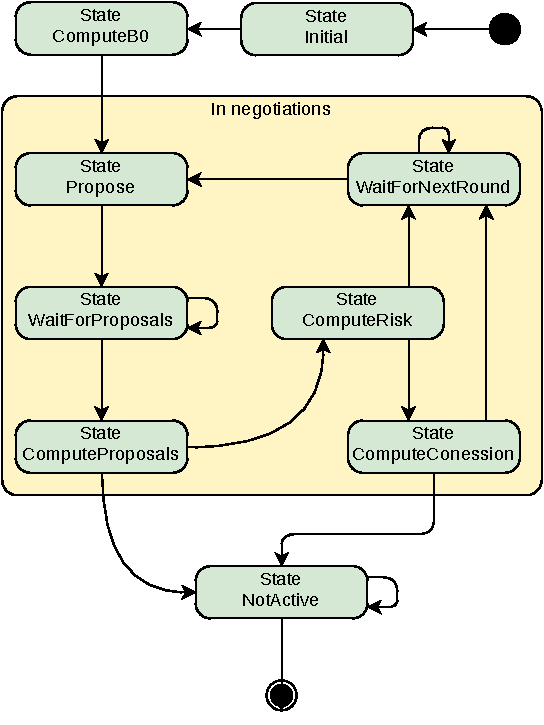
\includegraphics[width=0.53\columnwidth]{figures/SAG-FactoryFSM.pdf}
        \label{fig:factory-fsm}
    \end{figure}
\end{frame}


\section{Mechanizmy zabezpieczające}
\begin{frame}
    \frametitle{Założenia mechanizmów odpornościowych}

\end{frame}

\begin{frame}
    \frametitle{Rozszerzenia agentów o~zachowania zabezpieczające}
    \begin{figure}[!ht]
        \subfloat{%
            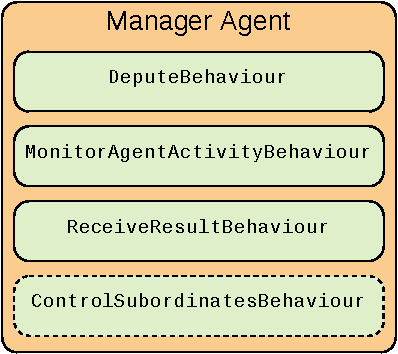
\includegraphics[width=0.54\columnwidth]{figures/SAG-Manager-Behaviours-Recovery.pdf}
        }
        \subfloat{%
            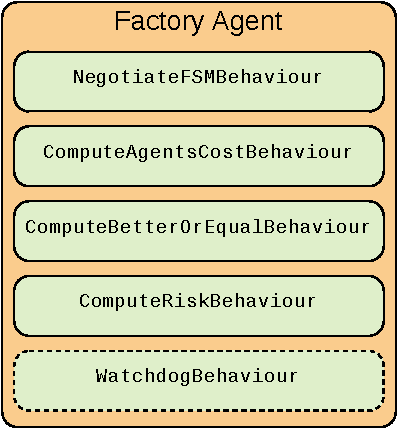
\includegraphics[width=0.46\columnwidth]{figures/SAG-Factory-Behaviours-Recovery.pdf}
        }
    \end{figure}
\end{frame}


\section{Skalowanie rozwiązania}
\begin{frame}
    \frametitle{Rozszerzenia systemu}

\end{frame}

\section{Podsumowanie}
\begin{frame}
    \frametitle{Podsumowanie}
    W~ramach projektu z~przedmiotu SAG udało się zrealizować:
    \begin{itemize}
        \item sam nwm
    \end{itemize}
\end{frame}

\end{document}
